\documentclass[aps,prd,twocolumn,superscriptaddress,nofootinbib,longbibliography,floatfix]{revtex4-2}

\usepackage{amsmath,amssymb,bm,mathtools,booktabs,microtype,graphicx}
\usepackage[colorlinks=true,allcolors=blue]{hyperref}
\newcommand{\Mpl}{\bar M_{\rm P}}
\newcommand{\dd}{\mathrm d}
\newcommand{\cM}{\mathcal M}
\newcommand{\cH}{\mathcal H}
\newcommand{\CP}{\mathbb{CP}}
\usepackage{orcidlink}
\IfFileExists{minimal_per_k_kernel_values.tex}{% Automatically generated by minimal_per_k_kernel.py
\newcommand{\PerKThirtyThreeInside}{93.2}
\newcommand{\PerKOneFiveInside}{22.3}
\newcommand{\PerKSthreeInside}{4.7}
\newcommand{\PerKThirtyThreeRMS}{0.002}
\newcommand{\PerKOneFiveRMS}{0.013}
\newcommand{\PerKSthreeRMS}{0.066}
}{}
\IfFileExists{matrix_per_k_kernel_values.tex}{% Automatically generated by matrix_per_k_kernel.py
\newcommand{\MatrixThirtyThreeInside}{67.8}
\newcommand{\MatrixThirtyThreeMinEig}{2.49e-07}
\newcommand{\MatrixThirtyThreeNs}{0.9695}
\newcommand{\MatrixThirtyThreeMaxResidual}{0.133}
\newcommand{\MatrixOneFiveInside}{47.8}
\newcommand{\MatrixOneFiveMinEig}{2.49e-07}
\newcommand{\MatrixOneFiveNs}{0.9811}
\newcommand{\MatrixOneFiveMaxResidual}{0.647}
\newcommand{\MatrixSthreeInside}{61.1}
\newcommand{\MatrixSthreeMinEig}{2.49e-07}
\newcommand{\MatrixSthreeNs}{0.9733}
\newcommand{\MatrixSthreeMaxResidual}{0.344}
}{}

% The REVTeX/BibTeX control entry below is used only to force article titles in the bibliography.
% It is not a reference, so define a dummy natbib label to avoid an undefined-citation warning.
\makeatletter
\@namedef{b@REVTEX42Control}{{}{}}{{}}{{}}
\makeatother

\begin{document}
\title{Lorentzian Boundary Kernels as a Compactification Test for Primordial Cosmology}

\author{Edward J. Shaya\ \orcidlink{0000-0002-3234-8699}}
\email{eshaya2@gmail.com}
\affiliation{Department of Astronomy, University of Maryland, College Park, USA}



\date{\today}

\begin{abstract}
A proposed higher-dimensional universe is usually tested against the cosmic microwave background only after a complete four-dimensional effective theory has been constructed, canonically normalized, and evolved mode by mode. We formulate a complementary test in which the primary object is the constrained Lorentzian boundary kernel of the Feynman--DeWitt wave functional. At quadratic order the imaginary part of this kernel is the inverse covariance of the physical boundary perturbations. The scalar and tensor power spectra, their tilts, the tensor-to-scalar ratio, isocurvature power, and stability conditions can therefore be read from one matrix-valued object. Heavy moduli and Kaluza--Klein modes enter through a Schur complement, which makes their decoupling or observational imprint explicit before a full Boltzmann analysis is attempted. We derive the general construction, recover the standard inflationary result in the single-field limit, and give two worked compactification templates: $M_4\times S^2 \times \CP^2$, including the flux branches $(m,n)=(3,3)$ and $(1,5)$, and $M_4 \times S^3\times S^3$ as a geometrically distinct control. The method does not uniquely reconstruct an internal manifold from the CMB. It provides a rapid acceptability test and a discriminant whenever internal modes remain light enough to modify the scalar or tensor kernel.
\end{abstract}

\maketitle

\section{Introduction}
The usual route from a higher-dimensional theory to a prediction for the cosmic microwave background (CMB) is conceptually straightforward but technically expensive. One chooses a compactification, reduces the theory to four dimensions, identifies the light fields, transforms to the four-dimensional Einstein frame, diagonalizes the kinetic terms, finds an inflationary background, derives the gauge-invariant perturbation equations, selects a quantum state, evolves every relevant mode, and finally passes the primordial spectra to a Boltzmann code. This sequence is necessary for precision parameter estimation. It is often more work than is needed to decide whether a candidate universe is viable at all.

This paper develops a faster intermediate test. The central object is the quadratic boundary kernel of the Lorentzian Feynman--DeWitt wave functional. The kernel is evaluated on the classical saddle after the lapse, shift, gauge redundancy, and nondynamical matter variables have been eliminated. Its imaginary part determines the Gaussian width of the physical boundary state. In Fourier space that width is the primordial covariance. In a coupled system the kernel is a matrix containing the curvature perturbation, the two graviton polarizations, isocurvature fields, moduli, and any Kaluza--Klein (KK) modes retained in the truncation.

The method is not a replacement for standard cosmological perturbation theory. At quadratic order it is the same physics written in a form particularly well adapted to comparing compactifications. The advantage is organizational. All effects of the internal manifold enter through four ingredients: the background saddle, the kinetic metric of the light fields, the mass and mixing matrices, and the spectrum of internal differential operators. These ingredients flow into a single effective boundary kernel. A compactification can be quickly shown to be consistent with present day observations of the CMB, or it can fail quickly because the kernel has a negative-width direction, an unsuppressed isocurvature eigenmode, an unacceptable scalar tilt, an excessive tensor amplitude, or a light internal mode that produces large features.

The formulation adopted here is therefore not proposed as an alternative quantum theory. For a fixed background sector, contour, and Gaussian state, it is equivalent to the Schrödinger wave functional, canonical mode-function quantization, and the in-in formalism. Its value lies in the way it organizes the problem. The classical solution appears as a saddle of the action, while the quadratic boundary Hessian records the finite quantum width around that saddle. Compactification moduli, KK modes, and observable perturbations can consequently be assembled into one matrix kernel and reduced uniformly before comparison with cosmological data. This representation may become especially useful when several fields, compactification sectors, or saddles must be retained simultaneously.

The uncertainty principle and inflationary mode evolution are likewise not treated as two independent stochastic mechanisms. In the Gaussian approximation they are, respectively, the width of the quantum state and the subsequent dynamical evolution of that same width. Inflation does not generate statistically independent fluctuations point by point; it evolves a correlated field configuration whose covariance is encoded by the boundary kernel. This viewpoint changes no quadratic prediction, but it makes explicit which information belongs to the state, which belongs to propagation, and which assumptions enter when a particular compactification and contour are selected.

The relation between a Gaussian wave functional and a cosmological spectrum is standard \cite{HalliwellHawking1985,PolarskiStarobinsky1996,Maldacena2003}. The useful point here is to treat the constrained matrix kernel as a common interface between higher-dimensional geometry and CMB observables. The same formula applies when one changes the compactification manifold, flux sector, or modulus content. In the decoupling limit all acceptable compactifications reduce to the familiar four-dimensional result. A manifold can be distinguished only through corrections that survive in the observable window.

We illustrate the procedure with two ten-dimensional products. The first is
\begin{equation}
\cM_{10}=M_4\times S^2\times\CP^2,
\end{equation}
which is the compactification used in the companion UECKK construction, the associated zero-mode family calculation, and the spin--torsion vacuum-stability analysis \cite{ShayaUECKK2026,ShayaZeroModes2026,ShayaVacuum2026}. It has independent radii and quantized fluxes. It admits the factorized chiral index
\begin{equation}
N_{\rm fam}=m\frac{n^2-1}{8},
\end{equation}
so that both $(m,n)=(3,3)$ and $(1,5)$ yield three chiral families while distributing the flux and zero-mode wave functions differently over the two factors. The second example is
\begin{equation}
\cM_{10}=M_4\times S^3\times S^3,
\end{equation}
which has a different curvature, harmonic spectrum, and modulus structure but remains simple enough to display the kernel construction analytically. It serves as a control rather than as a complete particle-physics model.

\section{The constrained Lorentzian boundary kernel}
\label{sec:kernel}

\subsection{Wave functional and saddle width}
Let $q_A(\bm x)$ denote a complete set of physical boundary variables on a spacelike hypersurface $\Sigma$. Before reduction, these variables are drawn from the induced spatial metric, matter fields, and internal metric components. The Feynman--DeWitt wave functional is
\begin{equation}
\Psi[q]=\int_{Q|_\Sigma=q}\mathcal DQ\,
\exp\left(\frac{i}{\hbar}S[Q]\right),
\end{equation}
where $Q$ collectively denotes bulk geometries and matter histories. The boundary data $q$ are not the bulk integration variables. They label the state obtained after the bulk histories have been summed.

Suppose the integral is dominated by a saddle $\bar Q$ and write $Q=\bar Q+\eta$. After gauge fixing and elimination of constraints, the action has the quadratic expansion
\begin{equation}
S[\bar Q+\eta]=S[\bar Q]+\frac12\eta\cdot\mathcal A\cdot\eta+\cdots .
\end{equation}
The contour that defines the state selects a generally complex solution of the linearized equations. Evaluating the quadratic action on that solution gives a boundary term,
\begin{equation}
S_{\rm os}^{(2)}[q]=\frac12\int\frac{\dd^3k}{(2\pi)^3}
q_A(-\bm k)K_{AB}(k)q_B(\bm k).
\label{eq:onshell}
\end{equation}
The matrix $K_{AB}$ is the Dirichlet-to-Neumann map: it converts the boundary amplitude into the canonical momentum of the regular bulk solution,
\begin{equation}
K_{AB}(k)=\left.\frac{\delta\Pi_A(\bm k)}{\delta q_B(\bm k)}\right|_\Sigma.
\end{equation}

Write $K=K_R+iK_I$, with $K_I$ Hermitian. Then
\begin{equation}
|\Psi[q]|^2\propto
\exp\left[-\frac1\hbar\int\frac{\dd^3k}{(2\pi)^3}
q_A(-\bm k)(K_I)_{AB}q_B(\bm k)\right].
\end{equation}
A normalizable Gaussian requires $K_I$ to be positive definite on the physical subspace. The covariance is
\begin{equation}
\langle q_A(\bm k)q_B(\bm k')\rangle
=(2\pi)^3\delta^3(\bm k+\bm k')\frac\hbar2(K_I^{-1})_{AB}.
\label{eq:cov}
\end{equation}
Equation~\eqref{eq:cov} is the central diagnostic of this paper.

The interpretation is elementary. The saddle is the mean history. The quadratic neighborhood of the saddle is its quantum width. In canonical language the uncertainty relation fixes an irreducible phase-space area, while the Hessian and the contour determine the shape and orientation of the uncertainty ellipse. The path integral does not assign independent random numbers to spatial cells; it assigns an amplitude to an entire constrained field configuration. A $1/\sqrt N$ counting law appears only when a coarse-grained observable averages over approximately independent correlation volumes.

\subsection{Constraints and physical variables}
For gravity the ADM action has the form
\begin{equation}
S=\int\dd t\,\dd^3x\left[\pi^{ij}\dot h_{ij}+p_I\dot\phi^I-N\mathcal H-N^i\mathcal H_i\right].
\end{equation}
The lapse and shift are Lagrange multipliers. Their functional integration enforces the Hamiltonian and momentum constraints. At the linearized level these constraints remove scalar and vector gauge directions and relate matter and metric perturbations. A practical calculation may solve the constraints before the path integral or integrate over nondynamical variables directly; both procedures give the same reduced kernel when the measure is treated consistently.

For an isotropic four-dimensional background with scalar fields $\varphi^a$, a convenient physical basis is
\begin{equation}
q_A=(\zeta,s^\alpha,h_+,h_\times,\chi^r),
\end{equation}
where $\zeta$ is the adiabatic curvature perturbation, $s^\alpha$ are isocurvature directions, $h_\lambda$ are the two tensor polarizations, and $\chi^r$ are retained internal or KK modes. The kernel in this basis is gauge invariant. A negative eigenvalue of $K_I$ is not a coordinate instability; it signals that the selected contour does not define a normalizable state in that direction or that the saddle is unstable.

\subsection{Moving the boundary}
The division between an ``initial state'' and ``later mode evolution'' depends on where an intermediate hypersurface is placed. Let $G_{21}(q_2,q_1)$ be the quadratic propagator between two boundaries. Composition gives
\begin{equation}
\Psi_2(q_2)=\int\mathcal Dq_1\,G_{21}(q_2,q_1)\Psi_1(q_1).
\end{equation}
For Gaussian kernels this integration is exact. If
\begin{equation}
S_{21}^{(2)}=\frac12q_2Aq_2+q_2Bq_1+\frac12q_1Cq_1
\end{equation}
and the earlier state has kernel $K_1$, then, up to convention-dependent factors of $i$,
\begin{equation}
K_2=A-B(C+K_1)^{-1}B^T.
\label{eq:compose}
\end{equation}
Moving the intermediate boundary changes $K_1$ and the propagator separately but not the final state. One may therefore place the numerical boundary where the effective description is best controlled and evolve the kernel rather than repeatedly re-quantizing the system.

\section{CMB observables from the kernel}
\label{sec:observables}

For the curvature perturbation,
\begin{equation}
\langle\zeta_{\bm k}\zeta_{\bm k'}\rangle
=(2\pi)^3\delta^3(\bm k+\bm k')P_\zeta(k),
\end{equation}
\begin{equation}
\Delta_\zeta^2(k)=\frac{k^3}{2\pi^2}P_\zeta(k).
\end{equation}
If all nonadiabatic modes have been integrated out,
\begin{equation}
P_\zeta(k)=\frac{\hbar}{2\,\operatorname{Im}K_{\zeta,\rm eff}(k)}.
\label{eq:pzeta}
\end{equation}
The amplitude, tilt, and running follow from
\begin{align}
A_s&=\Delta_\zeta^2(k_*),\\
n_s-1&=\left.\frac{\dd\ln\Delta_\zeta^2}{\dd\ln k}\right|_{k_*},\\
\alpha_s&=\left.\frac{\dd n_s}{\dd\ln k}\right|_{k_*}.
\end{align}

For the two graviton polarizations,
\begin{equation}
\Delta_T^2(k)=\frac{k^3}{2\pi^2}\sum_{\lambda=+,\times}P_{h_\lambda}(k),
\end{equation}
where each covariance is obtained from the inverse tensor block of $K_I$. The tensor-to-scalar ratio and tensor tilt are
\begin{equation}
r(k)=\frac{\Delta_T^2(k)}{\Delta_\zeta^2(k)},\qquad
n_T=\frac{\dd\ln\Delta_T^2}{\dd\ln k}.
\end{equation}
These quantities are especially useful compactification diagnostics because internal geometry can modify the scalar and tensor blocks differently. A shift in $A_s$ can often be absorbed into a change of the inflationary potential. A scale-dependent $r$, extra tensor polarizations, or a violation of $r=-8n_T$ is harder to imitate.

For rapid screening we use
\begin{equation}
A_s\simeq2.1\times10^{-9},\qquad
0.955<n_s<0.980,\qquad r_{0.05}<0.036,
\label{eq:screen}
\end{equation}
consistent with Planck and BICEP/Keck analyses \cite{PlanckInflation2020,BICEPKeck2021,BICEPKeckReview2024}. These are not a substitute for a likelihood analysis; they are pass/fail benchmarks.

\subsection{Recovery of the standard result}
The reduced quadratic action for a single adiabatic mode is
\begin{equation}
S_\zeta^{(2)}=\frac12\int\dd\eta\,\frac{\dd^3k}{(2\pi)^3}z^2
\left(|\zeta_k'|^2-c_s^2k^2|\zeta_k|^2\right),
\end{equation}
where $z^2=2a^2\epsilon\Mpl^2/c_s^2$. For canonical slow roll, $c_s=1$. In approximate de Sitter space, $a=-1/(H\eta)$, and the regular solution may be normalized as
\begin{equation}
u_k(\eta)=(1-ik\eta)e^{ik\eta}.
\end{equation}
The boundary kernel is $K_\zeta=z^2u_k'/u_k$, giving
\begin{equation}
\operatorname{Im}K_\zeta(k,\eta)=
\frac{2\epsilon\Mpl^2}{H^2}\frac{k^3}{1+k^2\eta^2}.
\end{equation}
At late times $|k\eta|\ll1$,
\begin{equation}
\operatorname{Im}K_\zeta\longrightarrow
\frac{2\epsilon\Mpl^2}{H^2}k^3.
\end{equation}
Equations~\eqref{eq:cov} and \eqref{eq:pzeta} then give
\begin{equation}
\Delta_\zeta^2=\frac{\hbar H_*^2}{8\pi^2\epsilon_*\Mpl^2},
\end{equation}
while the tensor block gives
\begin{equation}
\Delta_T^2=\frac{2\hbar H_*^2}{\pi^2\Mpl^2},\qquad r=16\epsilon_*.
\end{equation}
The method therefore reproduces the textbook answer. Its value is not a different prediction in the decoupling limit, but a cleaner route for deciding when a compactification does not lie in that limit.

\section{How compactification data enter}
\label{sec:compactification}

Consider a $D=4+d$ dimensional metric
\begin{equation}
\dd s_D^2=e^{2A(\phi)}g_{\mu\nu}(x)\dd x^\mu\dd x^\nu+G_{mn}(y;\phi)\dd y^m\dd y^n,
\end{equation}
where $\phi^a(x)$ are breathing, shape, and flux-supported moduli. In the four-dimensional Einstein frame,
\begin{equation}
S_4=\int\dd^4x\sqrt{-g}\left[\frac{\Mpl^2}{2}R-
\frac12G_{ab}(\phi)\partial_\mu\phi^a\partial^\mu\phi^b-V_{\rm eff}(\phi)\right]+S_{\rm light}.
\label{eq:einstframe}
\end{equation}

Fluctuations on the internal manifold are expanded in eigenfunctions of the appropriate scalar, vector, spinor, and Lichnerowicz operators. For a scalar harmonic,
\begin{equation}
-\nabla_{X_d}^2Y_I=\lambda_IY_I,\qquad
\chi(x,y)=\sum_I\chi_I(x)Y_I(y).
\end{equation}
The four-dimensional masses contain $\lambda_I$ plus curvature, flux, and interaction contributions. The internal geometry therefore enters through the spectral data $(\lambda_I,d_I)$ and overlap integrals that determine mixing.

Separate observable variables $L=(\zeta,h_+,h_\times)$ from internal variables $H=(s^\alpha,\chi^r)$. The quadratic boundary kernel is
\begin{equation}
K=\begin{pmatrix}K_{LL}&K_{LH}\\K_{HL}&K_{HH}\end{pmatrix}.
\end{equation}
Integrating out unobserved internal variables gives
\begin{equation}
K_{L,\rm eff}=K_{LL}-K_{LH}K_{HH}^{-1}K_{HL}.
\label{eq:schur}
\end{equation}
This Schur complement is the compactification correction. It contains changes in normalization, scale-dependent mixing, resonant structure, and the onset of instability when an eigenvalue of $K_{HH}$ approaches zero.

When an internal mode has mass $M\gg H$ and varies adiabatically,
\begin{equation}
\delta K_L\sim-\frac{K_{LH}K_{HL}}{M^2}
=\mathcal O\left(\frac{H^2}{M^2}\right)K_{LL},
\end{equation}
up to couplings and slow-roll factors. Distinct manifolds then become observationally degenerate. If $M\sim H$, corrections can be large and may appear in power-spectrum features or higher-point functions \cite{ArkaniHamedMaldacena2015}.

For numerical work one may evolve the kernel directly. For a canonically normalized vector $v$ obeying
\begin{equation}
v''+\Omega^2(k,\eta)v=0,
\end{equation}
let $F$ be a fundamental matrix of contour-selected solutions. The kernel is
\begin{equation}
K=F'F^{-1},
\end{equation}
up to the kinetic prefactor, and satisfies the Riccati equation
\begin{equation}
K'+K^2+\Omega^2=0.
\label{eq:riccati}
\end{equation}
This avoids separately normalizing every mixed mode and is convenient for scanning flux sectors or manifolds.

\section{Worked Example: $M_4\times S^2\times\CP^2$}
\label{sec:s2cp2}

\subsection{Background and flux branches}
Take the two-radius ansatz used in the UECKK and spin--torsion companion papers \cite{ShayaUECKK2026,ShayaVacuum2026},
\begin{equation}
\dd s_{10}^2=e^{2A}g_{\mu\nu}\dd x^\mu\dd x^\nu+a_1^2\dd\Omega_2^2+a_2^2\dd s_{\CP^2}^2,
\end{equation}
where the reference Fubini--Study metric is normalized once and all powers of $a_2$ are explicit. The internal volume scales as
\begin{equation}
V_6\propto a_1^2a_2^4.
\end{equation}
The two logarithmic radii may be written
\begin{equation}
u=\ln(a_1/a_{1,0}),\qquad v=\ln(a_2/a_{2,0}).
\end{equation}
These fields have the Einstein-frame kinetic metric derived in Appendix~\ref{app:unimodularG}. The important point is that unimodularity fixes the full spacetime measure, not the internal volume by itself. In the reduced phase-space treatment of unimodular quantum cosmology, for example, the unimodular constraint solves for the lapse in terms of the spatial volume while the spatial scale factor remains dynamical \cite{Yamashita2026UnimodularQC}. The ten-dimensional analogue is that a change of
\begin{equation}
\sigma=2u+4v=\ln(V_6/V_{6,0})
\end{equation}
can be compensated by the external determinant or lapse. Therefore the primary UECKK screening calculation retains the full two-radion metric. A fixed-internal-volume projection, with shape coordinate \(\chi=u-v\), is still useful as an optional truncation, but it is not the generic consequence of unimodularity.

A useful flux-and-curvature truncation is
\begin{equation}
\begin{split}
U(a_1,a_2)=&-A\left[\frac{2}{a_1^4a_2^4}+\frac{24}{a_1^2a_2^6}\right]\\
&+B\left[\frac{m^2}{2a_1^6a_2^4}+\frac{q n^2}{a_1^2a_2^8}\right]
-C\frac{N_{\rm fam}^2}{a_1^2a_2^4}.
\end{split}
\label{eq:potential}
\end{equation}
The first line is the internal-curvature contribution in the chosen reduction convention, the second contains quantized flux, and the final term is a volume-dependent attractive contribution. The coefficients $A,B,C,q$ are model parameters until derived from the microscopic action. The family index is
\begin{equation}
N_{\rm fam}=m\frac{n^2-1}{8}.
\end{equation}
Both $(3,3)$ and $(1,5)$ give $N_{\rm fam}=3$, but their flux terms are
\begin{align}
U_{\rm flux}^{(3,3)}&=B\left[\frac{9}{2a_1^6a_2^4}+\frac{9q}{a_1^2a_2^8}\right],\\
U_{\rm flux}^{(1,5)}&=B\left[\frac{1}{2a_1^6a_2^4}+\frac{25q}{a_1^2a_2^8}\right].
\end{align}
They therefore have different minima, modulus Hessians, and overlap tensors even though their net chiral family number is identical.

The first background test is algebraic:
\begin{equation}
\partial_{a_i}U=0,
\qquad
\text{eigenvalues}\left[G^{-1}\nabla\nabla U\right]>0.
\label{eq:backgroundtest}
\end{equation}
The first condition locates a compactification saddle; the second tests local stability in the homogeneous truncation. A negative eigenvalue rejects the branch before any CMB calculation.

\subsection{Internal spectra}
For a sphere of radius $a_1$, scalar harmonics obey
\begin{equation}
\lambda_{\ell}^{S^2}=\frac{\ell(\ell+1)}{a_1^2},\qquad d_\ell^{S^2}=2\ell+1.
\end{equation}
For the standard Fubini--Study normalization on $\CP^2$,
\begin{equation}
\lambda_p^{\CP^2}=\frac{4p(p+2)}{a_2^2},\qquad d_p^{\CP^2}=(p+1)^3,
\end{equation}
with a rescaling if a different curvature convention is used. Product harmonics have
\begin{equation}
\lambda_{\ell p}=\lambda_\ell^{S^2}+\lambda_p^{\CP^2}.
\end{equation}
Flux shifts the spectra of charged fields and changes the internal wave functions. That shift is essential for distinguishing $(3,3)$ from $(1,5)$: the branches have the same index but not the same mode profiles or mixing integrals.

\subsection{Quadratic kernel}
Retain the adiabatic mode, the two homogeneous moduli, and a finite set of KK modes,
\begin{equation}
q=(\zeta,u,v,h_+,h_\times,\chi_{\ell p}^{(r)}).
\end{equation}
After solving the four-dimensional lapse and shift constraints, the scalar block has the schematic action
\begin{equation}
S_S^{(2)}=\frac12\int\dd\eta\,\frac{\dd^3k}{(2\pi)^3}
\left[Q'^TQ'-Q^T\Omega_S^2(k,\eta)Q\right],
\end{equation}
where $Q$ is the canonically normalized scalar vector. The matrix $\Omega_S^2$ contains the field-space curvature, the canonically normalized Hessian of $U$, the KK eigenvalues, and mixing terms proportional to the turning rate of the background trajectory. The contour-selected fundamental matrix $F_S$ gives
\begin{equation}
K_S=F_S'F_S^{-1}.
\end{equation}
The effective curvature kernel follows from Eq.~\eqref{eq:schur}. The tensor block is computed independently, including any mixing of the four-dimensional graviton with internal transverse-traceless metric modes.

For a rapid branch comparison, define
\begin{equation}
\mathcal D_{(m,n)}(k)=\left\{
\operatorname{eig}K_I,\ A_s,\ n_s,\alpha_s,\ r,\ n_T,\beta_{\rm iso}
\right\}_{(m,n)}.
\end{equation}
The two branches are distinguishable only if
\begin{equation}
\mathcal D_{(3,3)}(k)\neq\mathcal D_{(1,5)}(k)
\end{equation}
by more than observational and theoretical uncertainties. If both modulus masses satisfy $M_u,M_v\gg H$ and all charged KK modes are heavier still, both branches reduce to the universal single-field kernel. The method then returns a useful null result: the CMB cannot discriminate the flux distribution at quadratic order.

\subsection{What can make the branches differ}
There are four leading possibilities. First, one branch may be unstable. Second, one may have a modulus with $M\sim H$, producing isocurvature or a scale-dependent Schur correction. Third, the time dependence of $V_6\propto a_1^2a_2^4$ may modify the tensor normalization through an evolving effective Planck mass. Fourth, flux-dependent KK levels may lie near $H$ and leave oscillatory or non-Gaussian signatures. The scalar power-law spectrum alone is unlikely to identify the branch if both are deep in the decoupling regime.

\section{$M_4\times S^3\times S^3$ as a control}
\label{sec:s3s3}

Consider
\begin{equation}
\dd s_{10}^2=e^{2A}g_{\mu\nu}\dd x^\mu\dd x^\nu+b_1^2\dd\Omega_{3,1}^2+b_2^2\dd\Omega_{3,2}^2.
\end{equation}
This product has the same number of internal dimensions as $S^2\times\mathbb{C}P^2$ but different curvature and spectral data. The internal volume scales as $b_1^3b_2^3$. Two logarithmic radii again give a volume and a shape mode.

For a unit three-sphere the scalar harmonics satisfy
\begin{equation}
\lambda_\ell^{S^3}=\frac{\ell(\ell+2)}{b^2},\qquad d_\ell^{S^3}=(\ell+1)^2.
\end{equation}
Product eigenvalues are
\begin{equation}
\lambda_{\ell_1\ell_2}=
\frac{\ell_1(\ell_1+2)}{b_1^2}+
\frac{\ell_2(\ell_2+2)}{b_2^2}.
\end{equation}
A stabilizing model may include curvature, a cosmological term, and quantized three-form flux on each factor. Its Einstein-frame potential can be written generally as
\begin{equation}
U_{33}(b_1,b_2)=U_{\rm curv}+U_{\rm flux}+U_{\rm other},
\end{equation}
with each term carrying a fixed power of $b_1$ and $b_2$ determined by dimensional reduction. The kernel algorithm is unchanged: locate a stable saddle, canonically normalize the two moduli, construct $\Omega^2$, solve the regular matrix mode problem, and take the Schur complement.

This control example makes the main methodological point. The observable formulas do not need to be reinvented. What changes is the internal input:
\begin{equation}
\begin{split}
\{G_{ab},U,\lambda_I,d_I,&\text{overlaps}\}_{S^2\times\CP^2} 
\longrightarrow \\
&\{G_{ab},U,\lambda_I,d_I,\text{overlaps}\}_{S^3\times S^3}.
\end{split}
\end{equation}
The same code then produces $K_{\zeta,\rm eff}$ and $K_{T,\rm eff}$. A proposed universe is rejected if either kernel fails the criteria below. If both manifolds pass and their internal modes decouple, their CMB two-point spectra are not a useful discriminant; one must turn to particle content, non-Gaussianity, or other observables.


\section{Numerical demonstration of the screening pipeline}
\label{sec:numericaldemo}
The preceding sections define a method, but a useful screening paper should also show that the chain from compactification data to an observational curve is operational. We therefore give a transparent benchmark calculation. The chosen dimensionless coefficients produce stable saddles and expose each computational step. They are not yet microscopic predictions of either compactification; a genuine verdict on a manifold requires coefficients and mixing matrices derived from its higher-dimensional action.

For a product of two Einstein spaces of dimensions $d_1$ and $d_2$, with logarithmic radii $\beta_i=\ln a_i$, the unconstrained Einstein-frame kinetic matrix in the homogeneous truncation is
\begin{equation}
G_{ij}=\Mpl^2\left(d_i\delta_{ij}+\frac12 d_i d_j\right).
\label{eq:kineticmatrixbenchmark}
\end{equation}
Thus, in units $\Mpl=1$,
\begin{equation}
G_{S^2\times\CP^2}=\begin{pmatrix}4&4\\4&12\end{pmatrix},\qquad
G_{S^3\times S^3}=\begin{pmatrix}15/2&9/2\\9/2&15/2\end{pmatrix}.
\end{equation}
For the illustrative benchmark in this section we keep the two-radion matrix. This is also the appropriate default for the UECKK interpretation used here: unimodularity fixes the total spacetime volume element and is normally solved by the lapse or determinant variable, not by freezing $V_6$. Appendix~\ref{app:unimodularG} derives this full metric and explains the optional fixed-internal-volume truncation. Appendix~\ref{app:canonicalmassscreen} gives the coordinate-invariant construction of the $G^{-1}H$ mass matrix and the optional one-field fixed-volume projection. The numerical decoupling table is placed here in the main text because it is part of the actual screening result, not a technical afterthought.
For $S^2\times\CP^2$ we set $A=B=q=1$ and $C=0.05$ in Eq.~\eqref{eq:potential}. For the control model we use
\begin{multline}
U_{33}=-6\left(b_1^{-5}b_2^{-3}+b_1^{-3}b_2^{-5}\right)\\
+\frac92\left(b_1^{-9}b_2^{-3}+b_1^{-3}b_2^{-9}\right)
+0.2\,b_1^{-3}b_2^{-3}.
\label{eq:s3benchmarkpotential}
\end{multline}
The extrema are found in logarithmic variables and the canonical mass matrix is $G^{-1}\nabla\nabla U$. Table~\ref{tab:benchmarknumbers} lists the results. All three examples possess a stable homogeneous saddle in this benchmark, but their radii and canonical mass eigenvalues differ substantially.

\begin{table}[tbp]
\caption{Dimensionless benchmark minima and eigenvalues of $G^{-1}\nabla\nabla U$. These values demonstrate the pipeline and are not microscopic predictions.}
\label{tab:benchmarknumbers}
\begin{ruledtabular}
\begin{tabular}{lcccc}
Model & $a_1$ or $b_1$ & $a_2$ or $b_2$ & $m_-^2$ & $m_+^2$\\
\hline
$(3,3)$ on $S^2\times\CP^2$ & 0.929 & 0.725 & 122.6 & 255.6\\
$(1,5)$ on $S^2\times\CP^2$ & 0.535 & 1.151 & 34.1 & 72.1\\
$S^3\times S^3$ control & 1.033 & 1.033 & 12.1 & 30.3\\
\end{tabular}
\end{ruledtabular}
\end{table}

The first CMB-scale use of these numbers is the decoupling test. At a stationary point the covariant mass matrix is
\begin{equation}
(M^2)^I{}_{J}=G^{IK}\nabla_K\nabla_JU=G^{IK}H_{KJ},
\qquad H_{KJ}=\partial_K\partial_JU,
\label{eq:maincanonicalmass}
\end{equation}
because the gradient of $U$ vanishes and the logarithmic-radion metric is constant. The dimensionless quantities that enter the per-$k$ kernel screen are
\begin{equation}
\mu_\pm^2=\frac{m_\pm^2}{H_*^2}.
\label{eq:mainmuratios}
\end{equation}
Table~\ref{tab:canonicalmasses} is therefore a main-text result: it gives the canonical masses consumed by the minimal per-$k$ implementation. The fixed-$V_6$ column is retained only as a diagnostic one-field truncation; it is not the default UECKK interpretation of unimodularity.

\begin{table}[tbp]
\caption{Canonical homogeneous-modulus masses for the benchmark $S^2\times\CP^2$ branches. The optional column $m_{\rm fixed\,V_6}^2$ is the one-field mass obtained only after imposing the additional fixed-internal-volume truncation. All entries use the same dimensionless potential units as Table~\ref{tab:benchmarknumbers}.}
\label{tab:canonicalmasses}
\begin{ruledtabular}
\begin{tabular}{c c c c c c}
branch & $a_1$ & $a_2$ & $m_-^2$ & $m_+^2$ & $m_{\rm fixed\,V_6}^2$\\
\hline
$(3,3)$ & $0.929$ & $0.725$ & $122.6$ & $255.6$ & $241.6$\\
$(1,5)$ & $0.535$ & $1.151$ & $34.1$ & $72.1$ & $72.0$
\end{tabular}
\end{ruledtabular}
\end{table}

\begin{figure*}[tbp]
\centering
\begin{minipage}{0.48\textwidth}
\centering
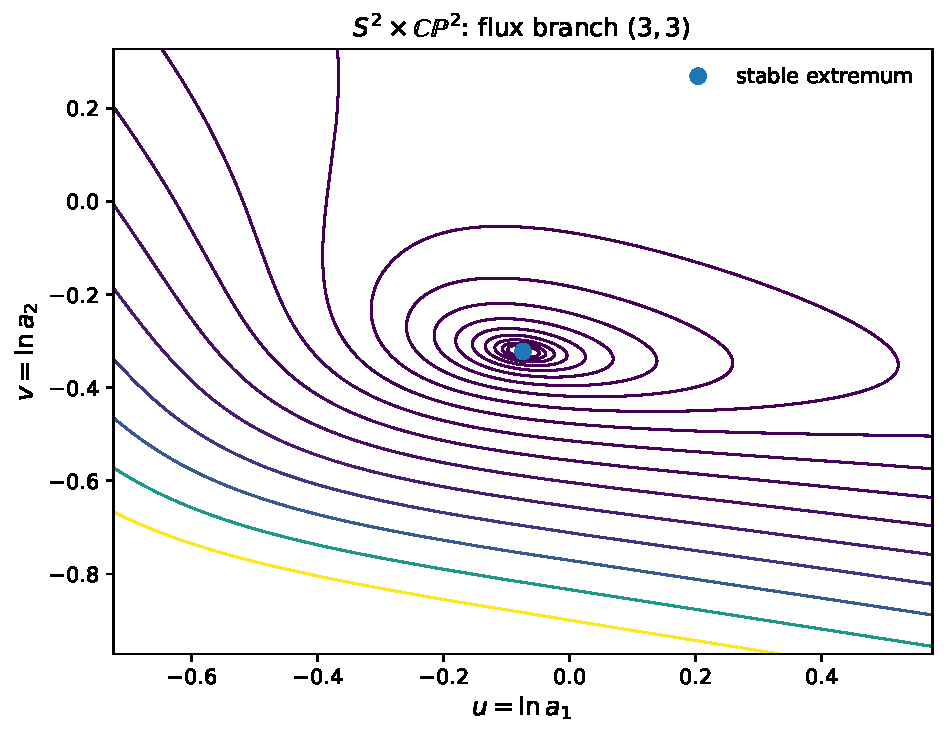
\includegraphics[width=\linewidth]{figures/benchmark_33.pdf}
\end{minipage}\hfill
\begin{minipage}{0.48\textwidth}
\centering
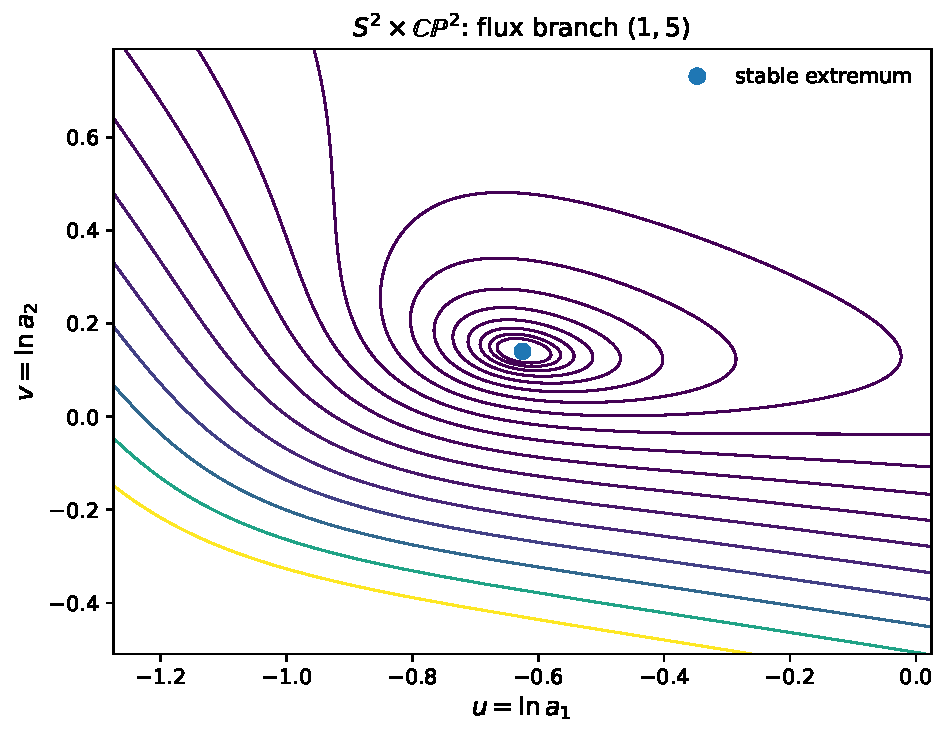
\includegraphics[width=\linewidth]{figures/benchmark_15.pdf}
\end{minipage}
\caption{Benchmark potentials for the two $S^2\times\CP^2$ branches. Left: $(3,3)$; right: $(1,5)$. The dots mark the stable extrema. Although the two branches have the same family index, their flux distributions move the minimum and change the local Hessian.}
\label{fig:benchmarkpotentials}
\end{figure*}

\subsection{Observed amplitude and the tensor constraint}
Combining $A_s=H_*^2/(8\pi^2\epsilon_*\Mpl^2)$ with $r=16\epsilon_*$ and $M_{\rm P}=\sqrt{8\pi}\Mpl$ gives
\begin{equation}
\frac{H_*}{M_{\rm P}}=\frac14\sqrt{\pi A_s r}.
\label{eq:Hrcurve}
\end{equation}
Figure~\ref{fig:amplitudecurve} uses $A_s=2.10\times10^{-9}$ and the BICEP/Keck limit $r_{0.05}<0.036$ \cite{BICEPKeck2021,BICEPKeckReview2024}. In the canonical single-field limit the bound corresponds to $H_*/M_{\rm P}<3.9\times10^{-6}$. A proposed compactification supplies the background value of $H_*$ and the tensor kernel supplies $r$; their point must lie on this curve.

\begin{figure}[tbp]
\centering
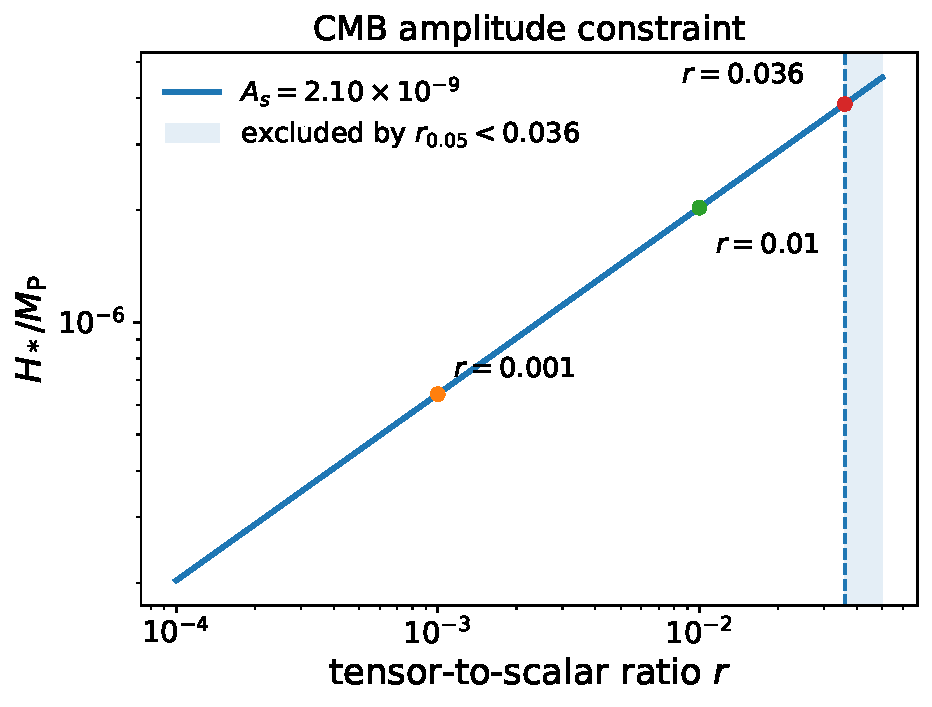
\includegraphics[width=\columnwidth]{figures/amplitude_curve.pdf}
\caption{The Hubble scale required by the measured scalar amplitude as a function of $r$. The shaded region is excluded by the current BICEP/Keck bound.}
\label{fig:amplitudecurve}
\end{figure}

\subsection{A one-mode Schur-complement visualization}
To display the last algebraic step, retain one internal scalar with dimensionless mass $\mu=M/H$ and approximate the imaginary kernel near the pivot by
\begin{equation}
\frac{\operatorname{Im}K_{\zeta,\rm eff}}{\operatorname{Im}K_{\zeta,0}}
=1-\frac{\gamma^2}{\mu^2+(k/k_*)^2}.
\label{eq:toySchur}
\end{equation}
Since the power is inversely proportional to $\operatorname{Im}K$, the response is
\begin{equation}
\frac{\Delta_\zeta^2}{\Delta_{\zeta,0}^2}
=\left[1-\frac{\gamma^2}{\mu^2+(k/k_*)^2}\right]^{-1}.
\end{equation}
For Fig.~\ref{fig:schurcorrection} we set the common illustrative values $H^2=10$ and $\gamma=0.4$, and insert the lighter canonical mass from Table~\ref{tab:benchmarknumbers}. The calculation is deliberately simple enough to reproduce by inspection. A full model replaces Eq.~\eqref{eq:toySchur} by the Riccati evolution of the constrained matrix kernel.

\begin{figure}[tbp]
\centering
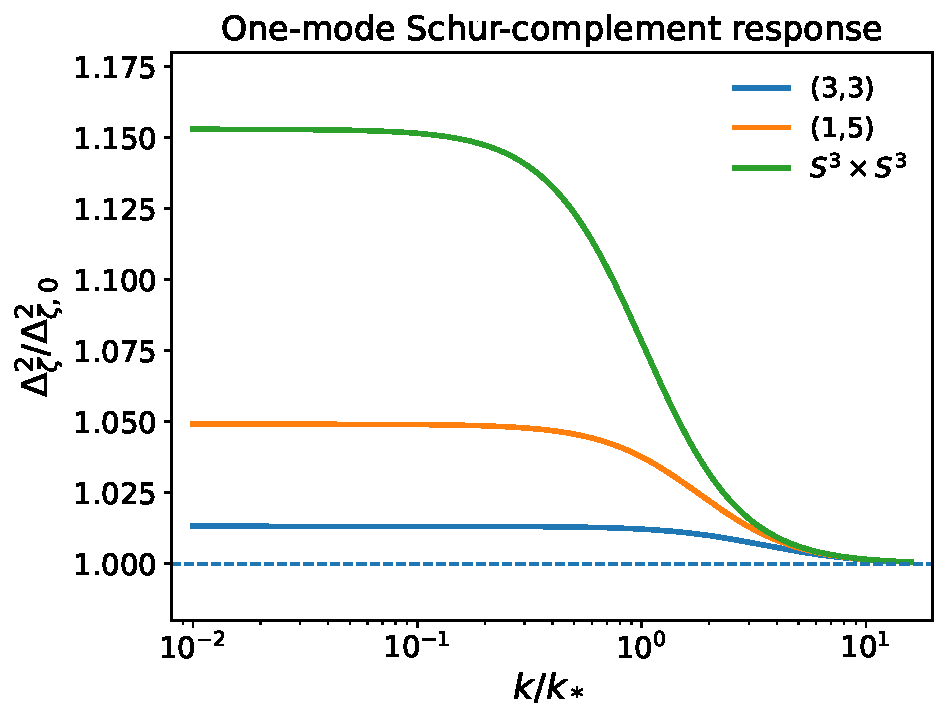
\includegraphics[width=\columnwidth]{figures/schur_corrections.pdf}
\caption{Illustrative scalar-power response from one internal mode. The different mass eigenvalues generate visibly different scale dependences.}
\label{fig:schurcorrection}
\end{figure}

\subsection{Direct comparison with the measured scalar spectrum}
Figure~\ref{fig:observationalcomparison} carries the benchmark through to an observational screen. The band is the pointwise envelope generated by the Planck 2018 constraints $n_s=0.9649\pm0.0042$ and $\ln(10^{10}A_s)=3.044\pm0.014$ \cite{PlanckParameters2020,PlanckInflation2020}. Each benchmark curve is normalized to the measured amplitude at $k_*=0.05\,\mathrm{Mpc}^{-1}$; the test therefore probes the additional scale dependence produced by the internal mode rather than refitting the amplitude.

With the illustrative choices above, the $(3,3)$ curve remains inside this one-standard-deviation parameter envelope over about $94\%$ of the plotted logarithmic $k$ grid, the $(1,5)$ curve over about $28\%$, and the $S^3\times S^3$ control over about $5\%$. These percentages are not likelihoods and must not be interpreted as observational confidence levels. They demonstrate that the kernel method can return a positive or negative screening verdict once the compactification masses and mixings are supplied. In this benchmark the $(3,3)$ branch is close to the observed power-law shape, whereas the lighter internal modes of the other examples generate excessive low-$k$ curvature.

\begin{figure*}[tbp]
\centering
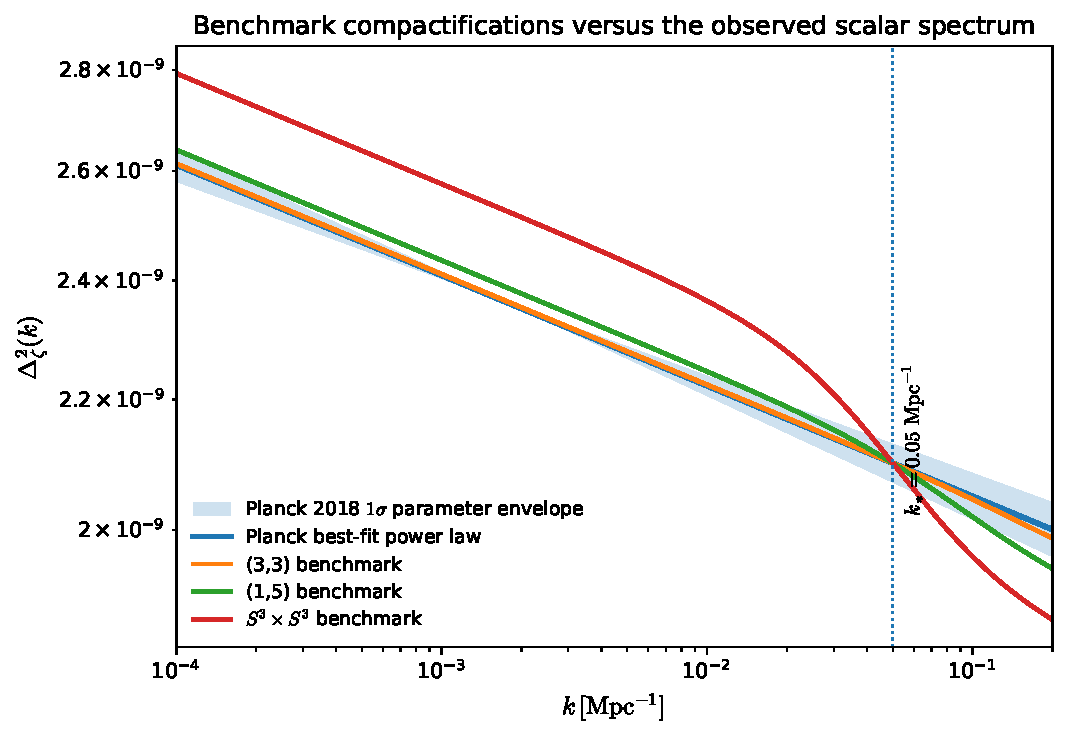
\includegraphics[width=0.88\textwidth]{figures/observational_comparison.pdf}
\caption{Benchmark primordial spectra compared with the Planck 2018 best-fit power law and its one-standard-deviation parameter envelope. This is an observational comparison, but not yet a manifold prediction: the benchmark mixing $\gamma$ and the overall potential normalization have not been derived from either higher-dimensional action. A genuine confirmation or exclusion of $M_4\times S^2\times\CP^2$ requires those microscopic inputs.}
\label{fig:observationalcomparison}
\end{figure*}

\begin{figure*}[tbp]
\centering
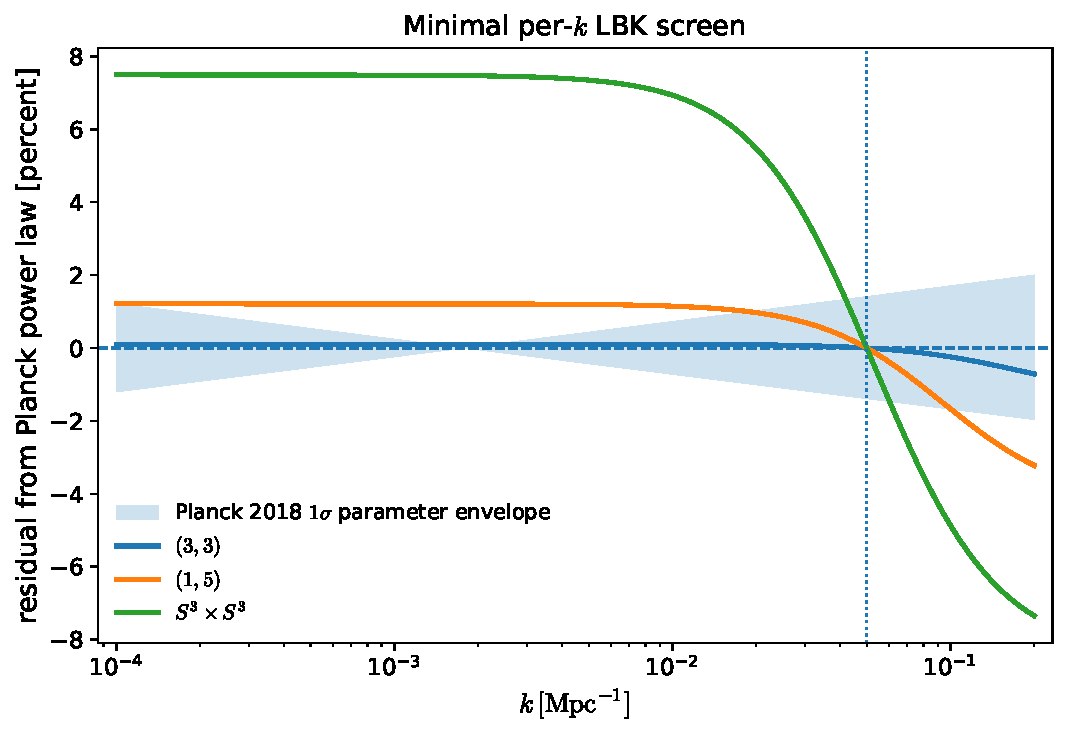
\includegraphics[width=0.88\textwidth]{figures/per_k_minimal_screen.pdf}
\caption{Minimal per-$k$ LBK implementation.  The curves show the fractional residual relative to the Planck best-fit primordial power law after pivot normalization.  The shaded region is the pointwise envelope generated by the $1\sigma$ uncertainties in $A_s$ and $n_s$.  For the illustrative choices $H^2=10$ and $\bm b=(0.40,0.22)$, the fractions of the plotted $k$ grid inside the envelope are $\PerKThirtyThreeInside\%$ for $(3,3)$, $\PerKOneFiveInside\%$ for $(1,5)$, and $\PerKSthreeInside\%$ for $S^3\times S^3$.  This is a code-level demonstration of the screening workflow, not a final Planck likelihood.}
\label{fig:perkminimal}
\end{figure*}

The comparison can be implemented literally as a loop over wavenumber.  For the minimal algebraic screen one sets $x=k/k_*$ and uses
\begin{equation}
R_{\mathcal M}(k)=\left[1-\bm b^{T}
\left(\operatorname{diag}\mu_a^2+x^2\mathbf 1\right)^{-1}\bm b\right]^{-1},
\qquad
\mu_a^2=\frac{m_a^2}{H_*^2},
\label{eq:perkresponse}
\end{equation}
where $m_a^2$ are the canonical hidden-sector eigenvalues and $\bm b$ is the dimensionless vector of curvature--modulus mixing strengths.  The primordial curve is then normalized at the pivot,
\begin{equation}
\Delta_{\zeta,\mathcal M}^2(k)=\Delta_{\zeta,\rm Pl}^2(k)
\frac{R_{\mathcal M}(k)}{R_{\mathcal M}(k_*)}.
\label{eq:perknormalized}
\end{equation}
Equations~\eqref{eq:perkresponse}--\eqref{eq:perknormalized} are the shortest useful implementation of the LBK screen for each $k$.  They do not replace the full Riccati evolution; rather, they provide a reproducible first pass that consumes the compactification masses and an assumed mixing vector before a full background trajectory is known.  The source package includes the script \texttt{minimal\_per\_k\_kernel.py}, which evaluates these equations on a logarithmic $k$ grid and writes Fig.~\ref{fig:perkminimal}.


\subsection{Matrix-evolved implementation of the per-$k$ workflow}
The algebraic screen above omits propagation.  We therefore also implement the matrix mode evolution listed in Appendix~\ref{app:numericalworkflow}.  The implementation retains one observable canonical mode and two hidden canonical modes.  For each $k$ it evolves a fundamental matrix $F$ in the variable $x=-k\eta$,
\begin{equation}
F_{,xx}+\left[\mathbf 1+\frac{C(x,k)}{x^2}\right]F=0,
\label{eq:matrixmodeimplementation}
\end{equation}
from the regular positive-frequency condition $F\propto e^{ix}\mathbf 1/\sqrt{2k}$.  The illustrative matrix $C$ contains the two canonical mass ratios and a localized curvature--modulus turn.  The turn is fixed in conformal time, so different wavenumbers encounter it at different values of $x$ and acquire a scale-dependent response.

At the final boundary the code constructs
\begin{equation}
K(k)=kF_{,x}F^{-1},
\qquad
K_{\zeta,\mathrm{eff}}=K_{\zeta\zeta}-K_{\zeta H}K_{HH}^{-1}K_{H\zeta},
\label{eq:implementedkernel}
\end{equation}
checks every eigenvalue of the Hermitian imaginary part of $K$, and compares $\operatorname{Im}K_{\zeta,\mathrm{eff}}$ with an otherwise identical zero-mixing evolution.  The resulting spectrum is normalized at the pivot before comparison with the Planck power law.

\begin{figure*}[tbp]
\centering
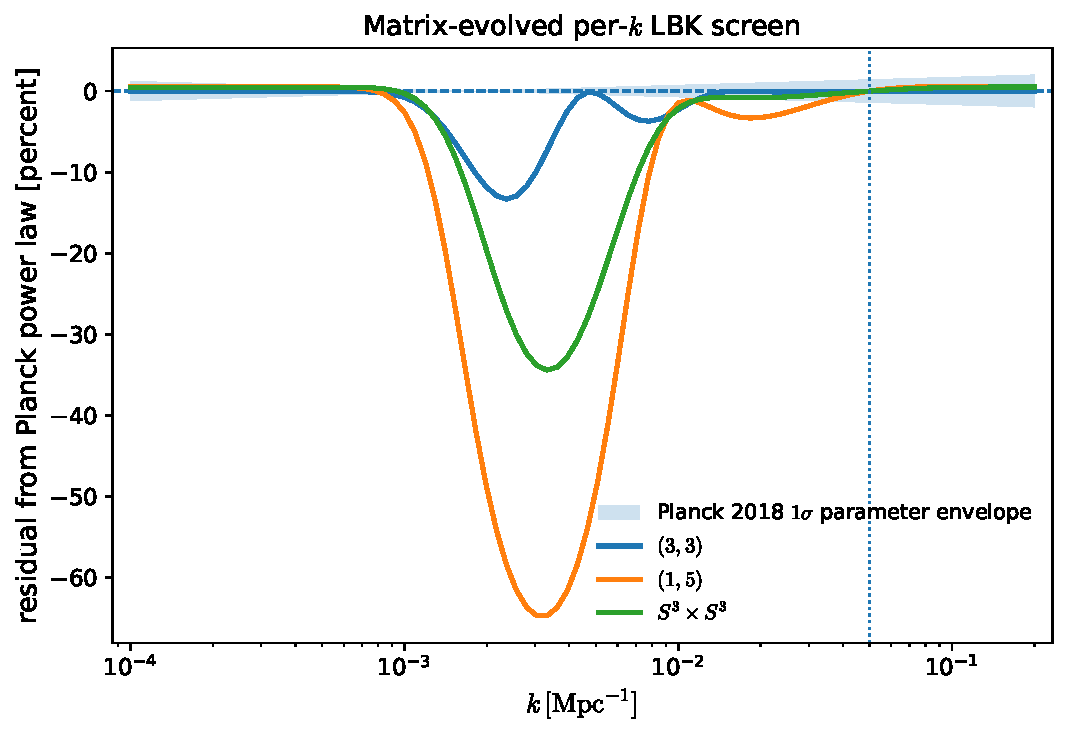
\includegraphics[width=0.88\textwidth]{figures/matrix_per_k_screen.pdf}
\caption{Dynamical matrix-mode implementation of the per-$k$ workflow.  Unlike Fig.~\ref{fig:perkminimal}, these curves follow from numerical evolution of a coupled fundamental matrix, construction of the late-time boundary kernel, a positivity check, and a Schur complement.  The localized turn and its mixing strengths remain illustrative rather than UECKK-derived.}
\label{fig:matrixperk}
\end{figure*}

\begin{table}[tbp]
\caption{Diagnostics from the matrix-evolved demonstration.  The effective tilt is fitted over $0.01\leq k\leq0.1\,{\rm Mpc}^{-1}$.  The final column is the largest absolute fractional departure from the pivot-normalized Planck power law over the plotted interval.}
\label{tab:matrixdiagnostics}
\begin{ruledtabular}
\begin{tabular}{lccc}
Model & inside [\%] & $n_s^{\rm eff}$ & max. residual\\
\hline
$(3,3)$ & $\MatrixThirtyThreeInside$ & $\MatrixThirtyThreeNs$ & $\MatrixThirtyThreeMaxResidual$\\
$(1,5)$ & $\MatrixOneFiveInside$ & $\MatrixOneFiveNs$ & $\MatrixOneFiveMaxResidual$\\
$S^3\times S^3$ & $\MatrixSthreeInside$ & $\MatrixSthreeNs$ & $\MatrixSthreeMaxResidual$\\
\end{tabular}
\end{ruledtabular}
\end{table}

For all three demonstrations the minimum eigenvalue of the imaginary kernel remains positive over the complete grid.  This verifies that the chosen contour and toy evolution define a normalizable Gaussian state.  The resulting percentages and tilts are not observational statements about the compactifications: they depend on the deliberately chosen turn profile.  Their purpose is narrower but concrete---every step of the proposed Appendix-D loop has now been executed in code.

The final qualification is essential. The present plot proves that the procedure works and shows which derived quantities control the answer. It does not yet provide positive evidence for the manifold, because changing the benchmark mixing changes the curves. A fourth companion paper on $M_4\times S^2\times\CP^2$ would become possible when $G_{ab}$, the full quadratic mixing matrix, and the inflationary trajectory are derived from the same microscopic model used in the family, torsion, and stability papers.

\section{A practical CMB acceptability test}
\label{sec:acceptance}

The boundary-kernel method is intended as a staged filter. It does not eliminate the final Boltzmann calculation for a successful model. It reduces the number of models that reach that stage.

\subsection{Stage 1: background viability}
For each manifold and flux sector:
\begin{enumerate}
\item Reduce to the four-dimensional Einstein frame and compute $G_{ab}(\phi)$ and $V_{\rm eff}(\phi)$.
\item Find a background solution with stabilized internal dimensions or a controlled slow trajectory.
\item Require positive kinetic eigenvalues and no tachyonic instability faster than the cosmological time scale.
\item Verify that the KK gap remains above the cutoff used in the truncation.
\end{enumerate}
A model failing this stage is not a candidate four-dimensional universe.

\subsection{Stage 2: kernel viability}
Construct the constrained scalar and tensor kernels on a grid of wavenumbers covering the observable CMB interval. Require
\begin{equation}
\operatorname{eig}K_I(k)>0
\end{equation}
for every retained physical mode and every relevant $k$. A zero or negative eigenvalue identifies a nonnormalizable direction, a bad contour choice, or a physical instability. Next integrate out modes not retained as observables and verify that the Schur complement is numerically stable.

\subsection{Stage 3: primordial observables}
From the effective kernels calculate
\begin{equation}
A_s,\quad n_s,\quad\alpha_s,\quad r,\quad n_T,
\quad\beta_{\rm iso},
\end{equation}
where $\beta_{\rm iso}$ is the fractional isocurvature power. Apply the broad windows in Eq.~\eqref{eq:screen} and an appropriately stringent isocurvature bound. A model passing these cuts is worth a full likelihood analysis.

\subsection{Stage 4: distinguishability}
For two candidate manifolds $\cM_1$ and $\cM_2$, define the fractional kernel separation
\begin{equation}
\Xi_X(k)=\frac{\left|\operatorname{Im}K_X^{(1)}(k)-
\operatorname{Im}K_X^{(2)}(k)\right|}
{\frac12\left[\operatorname{Im}K_X^{(1)}(k)+
\operatorname{Im}K_X^{(2)}(k)\right]},
\end{equation}
for $X=\zeta,T$. If $\Xi_X$ is smaller than the combined observational and theoretical uncertainty throughout the observable window, the two compactifications are CMB-degenerate at the level of two-point functions. This is not a failure of the method. It is the correct statement that the internal geometry has decoupled.

\begin{table*}[tbp]
\caption{Minimal inputs and outputs of the boundary-kernel screening test.}
\begin{ruledtabular}
\begin{tabular}{lll}
Stage & Required input & Immediate output\\
\hline
Background & $G_{ab}$, $V_{\rm eff}$, flux integers & stable saddle, $H(t)$, modulus masses\\
Internal spectrum & Laplace/Lichnerowicz eigenvalues and overlaps & KK masses, degeneracies, mixing matrices\\
Quadratic dynamics & constrained scalar and tensor actions & matrix frequencies $\Omega_S^2$, $\Omega_T^2$\\
Lorentzian state & regularity or $i\epsilon$ contour & positive imaginary boundary kernel\\
CMB screen & $K_{\zeta,\rm eff}$, $K_{T,\rm eff}$ & $A_s,n_s,\alpha_s,r,n_T,\beta_{\rm iso}$\\
Discrimination & two or more candidate kernels & exclusion, distinguishability, or decoupling bound\\
\end{tabular}
\end{ruledtabular}
\end{table*}

\section{Discussion}
\label{sec:discussion}

\subsection{What is new and what is not}
The identification of the Gaussian wave-functional width with the primordial covariance is not new. Neither is the standard inflationary result recovered in Sec.~\ref{sec:observables}. The proposed contribution is a calculational organization: the constrained Lorentzian boundary kernel is used as a common comparison object for candidate higher-dimensional universes. The same matrix formalism handles moduli, KK towers, scalar-tensor mixing, and boundary relocation.

This organization is useful only if it saves work or exposes a failure earlier than the conventional pipeline. The main savings are threefold. First, positivity of the imaginary kernel tests stability and normalizability before a full transfer-function calculation. Second, the Schur complement states immediately whether heavy internal modes decouple. Third, evolving a matrix Riccati equation can be simpler than separately normalizing a large set of coupled mode functions.

\subsection{Can the CMB determine the manifold?}
Generally no. Distinct manifolds can produce the same four-dimensional light theory, and even spectral data need not uniquely determine a geometry. The realistic outcomes are exclusion of a branch, distinction between broad classes, or constraints on modulus masses and couplings. The scalar two-point spectrum is already close to a featureless power law, so viable manifolds must reproduce nearly the same scalar kernel. Tensor modes, isocurvature, non-Gaussianity, and flux-dependent massive exchanges are more promising discriminants.

For the $(3,3)$ and $(1,5)$ branches, the family index alone cannot distinguish them. The difference lies in the flux distribution, the internal wave-function profiles, and the resulting modulus and KK kernels. If both branches have all internal masses far above $H$, the CMB cannot tell them apart at quadratic order. If one branch contains a mode near the Hubble scale, the method identifies the corresponding correction and indicates which observable should be computed next.

\subsection{Relation to an early high-curvature boundary}
The kernel formalism does not require the initial boundary to lie at a particular curvature. Moving an intermediate boundary merely redistributes the description between an assigned boundary state and subsequent propagation, provided the same contour and dynamics are used. A specific quantum-boundary proposal may supply a physical earliest surface, but it is not needed for the kernel method itself.

Similarly, a short decelerating period can lower a high initial Hubble rate before inflation, but that standard Friedmann scaling is not the source of the observed fractional perturbation amplitude. The amplitude is fixed by the kernel when observable modes exit the inflationary horizon, through the combination $H_*^2/\epsilon_*$. The present formalism cleanly separates that universal statement from compactification-specific dynamics.

\subsection{Limitations}
The method is semiclassical and quadratic. It assumes a controllable saddle, a well-defined contour, and a truncation whose omitted modes do not invalidate the Schur complement. A candidate passing the two-point test may still fail through non-Gaussianity, reheating, defects, late-time moduli, or particle-physics constraints. Near the compactification or quantum-gravity scale, higher-derivative operators and the full KK tower may be important. These are not technical footnotes: they define the domain in which the screening calculation is trustworthy.

\section{Conclusion}
A higher-dimensional cosmological model can be screened against the CMB through its constrained Lorentzian boundary kernel. The imaginary part of that kernel is the inverse covariance of the physical boundary variables. Scalar and tensor spectra are therefore read from the same object that tests stability and encodes mixing with internal modes.

The method reproduces the standard single-field inflationary spectrum when moduli and KK modes decouple. Its practical value appears away from that limit. For $M_4\times S^2\times\CP^2$, the $(3,3)$ and $(1,5)$ flux branches have the same chiral family index but different flux support, modulus Hessians, charged spectra, and overlap tensors. These differences enter the effective scalar and tensor kernels through a Schur complement. For $M_4\times S^3\times S^3$, the same algorithm applies with different curvature and harmonic data. No new cosmological formalism is required when the manifold is changed; only the internal inputs change.

The method is best viewed as an acceptability filter. It can reject unstable compactifications, identify light internal modes, quantify decoupling, and determine whether a full CMB likelihood calculation is warranted. It cannot generally infer a unique manifold from a nearly featureless scalar spectrum. A successful discrimination will most likely involve tensor modes, isocurvature, non-Gaussianity, or a characteristic departure from the four-dimensional consistency relations.

Equivalent formulations of a quantum theory need not be equally transparent for every problem. Canonical and in-in methods are particularly effective for perturbative evolution on a chosen background. The boundary-wave-functional representation instead emphasizes the global state, its contour and boundary data, and the possibility of combining multiple sectors or saddles before observables are extracted. At quadratic order these descriptions agree. Beyond that order, the same organization may help identify contributions that are easy to suppress when the background, state, topology, or compactification sector is fixed at the outset. Establishing whether any such contribution survives as a gauge-invariant observable is a separate problem, but the kernel hierarchy provides a natural framework in which to ask it.

\appendix
\section{Gaussian integration and the Schur complement}
Let a Gaussian state depend on observed variables $x$ and hidden variables $y$,
\begin{equation}
\Psi(x,y)\propto\exp\left[\frac{i}{2\hbar}
\begin{pmatrix}x&y\end{pmatrix}
\begin{pmatrix}A&B\\B^T&C\end{pmatrix}
\begin{pmatrix}x\\y\end{pmatrix}\right].
\end{equation}
Integrating over $y$ gives
\begin{equation}
\Psi_{\rm eff}(x)\propto
(\det C)^{-1/2}\exp\left[\frac{i}{2\hbar}x^T
\left(A-BC^{-1}B^T\right)x\right],
\end{equation}
with the contour chosen so that the Gaussian converges. This proves Eq.~\eqref{eq:schur}. For a field theory the matrices carry momentum labels and functional determinants replace ordinary determinants.




\section{Radion metric input for $S^2\times\CP^2$ and the role of unimodularity}
\label{app:unimodularG}
The full Einstein-frame reduction of the homogeneous $S^2\times\CP^2$ radii is part of the UECKK compactification analysis and is given in the companion construction \cite{ShayaUECKK2026}. Here we record only the result and the short derivation needed to make the LBK screening calculation self-contained.

Let
\begin{equation}
 u=\ln a_1,\qquad v=\ln a_2,
\end{equation}
where $a_1$ and $a_2$ are the radii of $S^2$ and $\CP^2$. For a product compactification with internal dimensions $d_i$, the four-dimensional Einstein-frame radion metric in logarithmic coordinates is
\begin{equation}
\mathcal G_{ij}=d_i\delta_{ij}+\frac{d_i d_j}{D_4-2}
=d_i\delta_{ij}+\frac12 d_i d_j,
\qquad D_4=4 .
\label{eq:generalradionmetric}
\end{equation}
Thus, for $d_1=2$ and $d_2=4$,
\begin{equation}
\boxed{
\mathcal G_{uv}=\begin{pmatrix}4&4\\4&12\end{pmatrix},
\qquad
G_{uv}=\Mpl^2\begin{pmatrix}4&4\\4&12\end{pmatrix}.
}
\label{eq:fullS2CP2G}
\end{equation}
The corresponding field-space line element is
\begin{equation}
\dd s_{\rm rad}^2=4\dd u^2+8\dd u\dd v+12\dd v^2.
\end{equation}
In volume and shape variables,
\begin{equation}
\sigma=2u+4v,\qquad \chi=u-v,
\end{equation}
one obtains
\begin{equation}
\dd s_{\rm rad}^2=\frac23\dd\sigma^2+\frac43\dd\chi^2.
\label{eq:diagvolshape}
\end{equation}

The unimodular condition fixes the full spacetime volume element, not the internal volume by itself. This distinction is visible already in reduced unimodular quantum cosmology: the condition fixes the product $Na^3$ and solves for the lapse, while the spatial scale factor remains dynamical \cite{Yamashita2026UnimodularQC}. In the present ten-dimensional product, a change in $a_1^2a_2^4$ can similarly be compensated by the external determinant or lapse. Therefore the default LBK screen uses the full two-radion metric in Eq.~\eqref{eq:fullS2CP2G}. A fixed-internal-volume line,
\begin{equation}
\delta\sigma=2\delta u+4\delta v=0,
\end{equation}
may be imposed as a separate truncation. Its induced metric is
\begin{equation}
\dd s_{\rm fixed\,V_6}^2=\frac43\dd\chi^2,
\qquad
G_{\chi\chi}^{\rm fixed\,V_6}=\frac43\Mpl^2,
\label{eq:Gchichi}
\end{equation}
but this is not the generic UECKK kinetic metric used below.

\section{Canonical modulus masses and the first CMB-scale screen}
\label{app:canonicalmassscreen}
The first compactification-level screen is the comparison between physical homogeneous-modulus masses and the inflationary scale. This appendix gives the coordinate-invariant construction using the full metric in Eq.~\eqref{eq:fullS2CP2G}. The fixed-internal-volume shape projection is included only as a diagnostic comparison.

Let
\begin{equation}
U(u,v)=\sum_A c_A\exp(-\alpha_A u-\beta_A v).
\end{equation}
The Hessian in logarithmic coordinates is
\begin{equation}
H_{IJ}=\partial_I\partial_JU
=\sum_A c_A
\begin{pmatrix}
\alpha_A^2&\alpha_A\beta_A\\
\alpha_A\beta_A&\beta_A^2
\end{pmatrix}
\exp(-\alpha_Au-\beta_Av),
\label{eq:fullHessianExp}
\end{equation}
with signs already squared by the second derivative. At a stationary point, connection terms in $\nabla_I\nabla_JU$ vanish; since the metric is constant in $(u,v)$, the physical mass matrix is simply
\begin{equation}
\boxed{
(M^2)^I{}_{J}=G^{IK}H_{KJ}
=\frac{1}{\Mpl^2}(\mathcal G^{-1})^{IK}H_{KJ}.
}
\label{eq:fullCanonicalMass}
\end{equation}
Its two eigenvalues $m_-^2$ and $m_+^2$ are the masses that should be compared with $H_*^2$ in the homogeneous-sector CMB screen.

For the illustrative coefficients used in Sec.~\ref{sec:numericaldemo}, $A=B=q=1$ and $C=0.05$, the resulting two-field masses are reported in Table~\ref{tab:canonicalmasses} in the main text, where they are used as the input to the per-$k$ screening calculation. The CMB-scale decoupling variables are those of Eq.~\eqref{eq:mainmuratios}.
A branch with both $\mu_\pm^2\gg1$ has no homogeneous-modulus isocurvature problem at quadratic order; the moduli decouple and the scalar spectrum approaches the universal four-dimensional result. A branch with one $\mu^2\sim1$ requires the full coupled kernel evolution because curvature--modulus mixing can generate scale dependence or residual isocurvature. A negative eigenvalue rejects the branch at the homogeneous level. After the microscopic normalization of $U$ is fixed by the UECKK action, Eq.~\eqref{eq:fullCanonicalMass} gives the physical ratios $m_\pm^2/H_*^2$.

For completeness, if one imposes the separate fixed-internal-volume truncation $\sigma=\sigma_0$, the pullback potential is
\begin{equation}
U_{\rm fixed\,V_6}(\chi)=U\left(\frac{\sigma_0}{6}+\frac{2\chi}{3},
\frac{\sigma_0}{6}-\frac{\chi}{3}\right).
\end{equation}
Then
\begin{equation}
 m_{\rm fixed\,V_6}^2
 =\frac{p^I H_{IJ}p^J}{\Mpl^2 p^I\mathcal G_{IJ}p^J},
\qquad
p^I=\left(\frac23,-\frac13\right),
\end{equation}
with $p^I\mathcal G_{IJ}p^J=4/3$. This diagnostic projection is not used in place of the full two-field screen unless fixed internal volume is imposed as an additional model assumption.

\section{Implemented numerical workflow}
\label{app:numericalworkflow}
The source package contains two executable levels of the screen.  The script \texttt{minimal\_per\_k\_kernel.py} evaluates the algebraic Schur-complement approximation in Eqs.~\eqref{eq:perkresponse}--\eqref{eq:perknormalized}.  The script \texttt{matrix\_per\_k\_kernel.py} follows through on the dynamical workflow and produces Fig.~\ref{fig:matrixperk}, Table~\ref{tab:matrixdiagnostics}, a CSV table, and the \LaTeX{} macros used in the main text.

For every wavenumber the implemented loop is:
\begin{enumerate}
\item read the canonical hidden-sector masses $\mu_a^2=m_a^2/H^2$;
\item assemble the symmetric coupled frequency matrix in Eq.~\eqref{eq:matrixmodeimplementation};
\item initialize the regular positive-frequency fundamental matrix at $x_i=60$;
\item evolve $F$ and $F_{,x}$ with an adaptive eighth-order Runge--Kutta integrator to $x_f=0.05$;
\item construct the boundary Dirichlet-to-Neumann matrix $K=kF_{,x}F^{-1}$;
\item form the Hermitian width matrix $K_I=(K-K^\dagger)/(2i)$ and require all of its eigenvalues to be positive;
\item integrate out the two hidden modes using the Schur complement in Eq.~\eqref{eq:implementedkernel};
\item repeat the evolution with the mixing set to zero, take the ratio of effective imaginary kernels, normalize it at $k_*$, and multiply the Planck power law by that response;
\item write the spectrum and diagnostics over a logarithmic grid from $10^{-4}$ to $0.2\,{\rm Mpc}^{-1}$.
\end{enumerate}

The illustrative frequency correction is
\begin{equation}
C(x,k)=
\begin{pmatrix}
-2 & g_1T(x,k) & g_2T(x,k)\\
g_1T(x,k) & \mu_1^2-2 & 0\\
g_2T(x,k) & 0 & \mu_2^2-2
\end{pmatrix},
\label{eq:toyfrequencycorrection}
\end{equation}
where
\begin{equation}
T(x,k)=\exp\left[-\frac{1}{2\sigma_T^2}
\ln^2\left(\frac{x/k}{|\eta_T|}\right)\right].
\label{eq:turnprofile}
\end{equation}
The numerical demonstration uses $|\eta_T|=k_*^{-1}$, $\sigma_T=0.55$, and $(g_1,g_2)=(0.05,0.025)$.  These values are exposed at the top of the script and are not fitted.  Replacing Eqs.~\eqref{eq:toyfrequencycorrection}--\eqref{eq:turnprofile} by the constrained scalar or tensor matrix derived from a compactification leaves the rest of the code path unchanged.

This implementation closes the gap between the formal prescription and an executable calculation, but it does not close the microscopic gap.  A physical UECKK run still requires the background trajectory, the canonically normalized curvature--radion mixing matrix, and any retained KK overlaps from the higher-dimensional action.  Once those are supplied, the toy frequency constructor is the only module that must be replaced.  A subsequent precision stage would pass the resulting scalar, tensor, and isocurvature spectra to CLASS or CAMB and evaluate a likelihood rather than the pointwise envelope used here.

\nocite{REVTEX42Control}
\bibliographystyle{apsrev4-2}
\bibliography{Lorentzian_Boundary_Kernels_PRD_References}

\end{document}
